\section{Auswertung}
\label{sec:Auswertung}
\subsection{Charakteristik des Geiger-Müller-Zählrohrs}

Es wird eine Thallium-Quelle verwendet. \\
Bei Aufnahme der Messwerte für die Charakteristik des Zählrohres wird 
die anliegende Spannung in $10$V-Schritten erhöht und bei einer Integrationszeit
von $120$s gemessen.\\
Ungewöhnlich weit abweichende Werte wurden in der Auswertung nicht berücksichtigt. In \autoref{tab:charak} 
sind die einbezogenen Messwerte zu finden. Der gesamte Satz an Messwerten ist in 
\autoref{sec:anhang} aufgelistet.\\

\begin{table}[H]
  \centering
  \caption{Die ausgewerteten Messwerte.}
  \begin{tabular}{ccc}
    \toprule
    {$U  \mathbin{/} \unit{\volt}$} &
    {$N \mathbin{/} \mathbin{Imp}$} &
    {$I \mathbin{/} \unit{\micro\ampere}$} \\
    \midrule
    330  &  12435 &  0.1   \\
    340  &  13454 &  0.1   \\
    350  &  13651 &  0.1   \\
    360  &  13660 &  0.1   \\
    370  &  13778 &  0.1   \\
    380  &  13770 &  0.1   \\
    390  &  13738 &  0.15  \\
    400  &  14003 &  0.15  \\
    410  &  14192 &  0.18  \\
    420  &  13730 &  0.2   \\
    430  &  14211 &  0.21  \\
    440  &  13861 &  0.21  \\
    480  &  14391 &  0.3   \\
    490  &  14047 &  0.3   \\
    500  &  14092 &  0.3   \\
    510  &  14164 &  0.3   \\
    520  &  14296 &  0.3   \\
    590  &  14337 &  0.4   \\
    600  &  14202 &  0.4   \\
    610  &  14087 &  0.45  \\
    620  &  14180 &  0.45  \\
    630  &  14290 &  0.47  \\
    640  &  14130 &  0.48  \\
    650  &  14466 &  0.5   \\
    660  &  14052 &  0.5   \\
    670  &  14170 &  0.5   \\
    680  &  14589 &  0.52  \\
    690  &  14653 &  0.6   \\
    700  &  14715 &  0.6   \\
    \bottomrule
  \end{tabular}
  \label{tab:charak}
\end{table}

Die Zählraten entsprechen einer Poisson-Verteilung, sodass sich ihr Fehler zu 
\begin{equation*}
  \Delta N = \sqrt{N}
\end{equation*}
ergibt.\\
Die Charakteristik ist in \autoref{fig:charakteristik} graphisch dargestellt.
Der Plateaubereich umfasst das Intervall von 410V bis 670V.\\
Die lineare Regression wird mithilfe von python (\cite{numpy}, \cite{uncertainties}) durchgeführt und ergibt
für die Ausgleichsgerade die Parameter $a = 0,73 \frac{\%}{100 V}$ für die Steigung und $b = 1376 \: Imp$ für den y-Achsenabschnitt.\\

\begin{figure}[H]
  \centering
  \includegraphics{content/figure_1_1.png}
  \caption{Die Charakteristik des Geiger-Müller-Zählrohrs.}
  \label{fig:charakteristik}
\end{figure}


\subsection{Bestimmung der Totzeit}
\subsubsection{Mit Oszilloskop}
Aus dem aufgenommenen Oszillogramm \autoref{fig:totzeit} kann zufolge xxx eine Totzeit von 
$T_1 = 150 \mu$s abgelesen werden..\\
\begin{figure}[H]
  \centering
  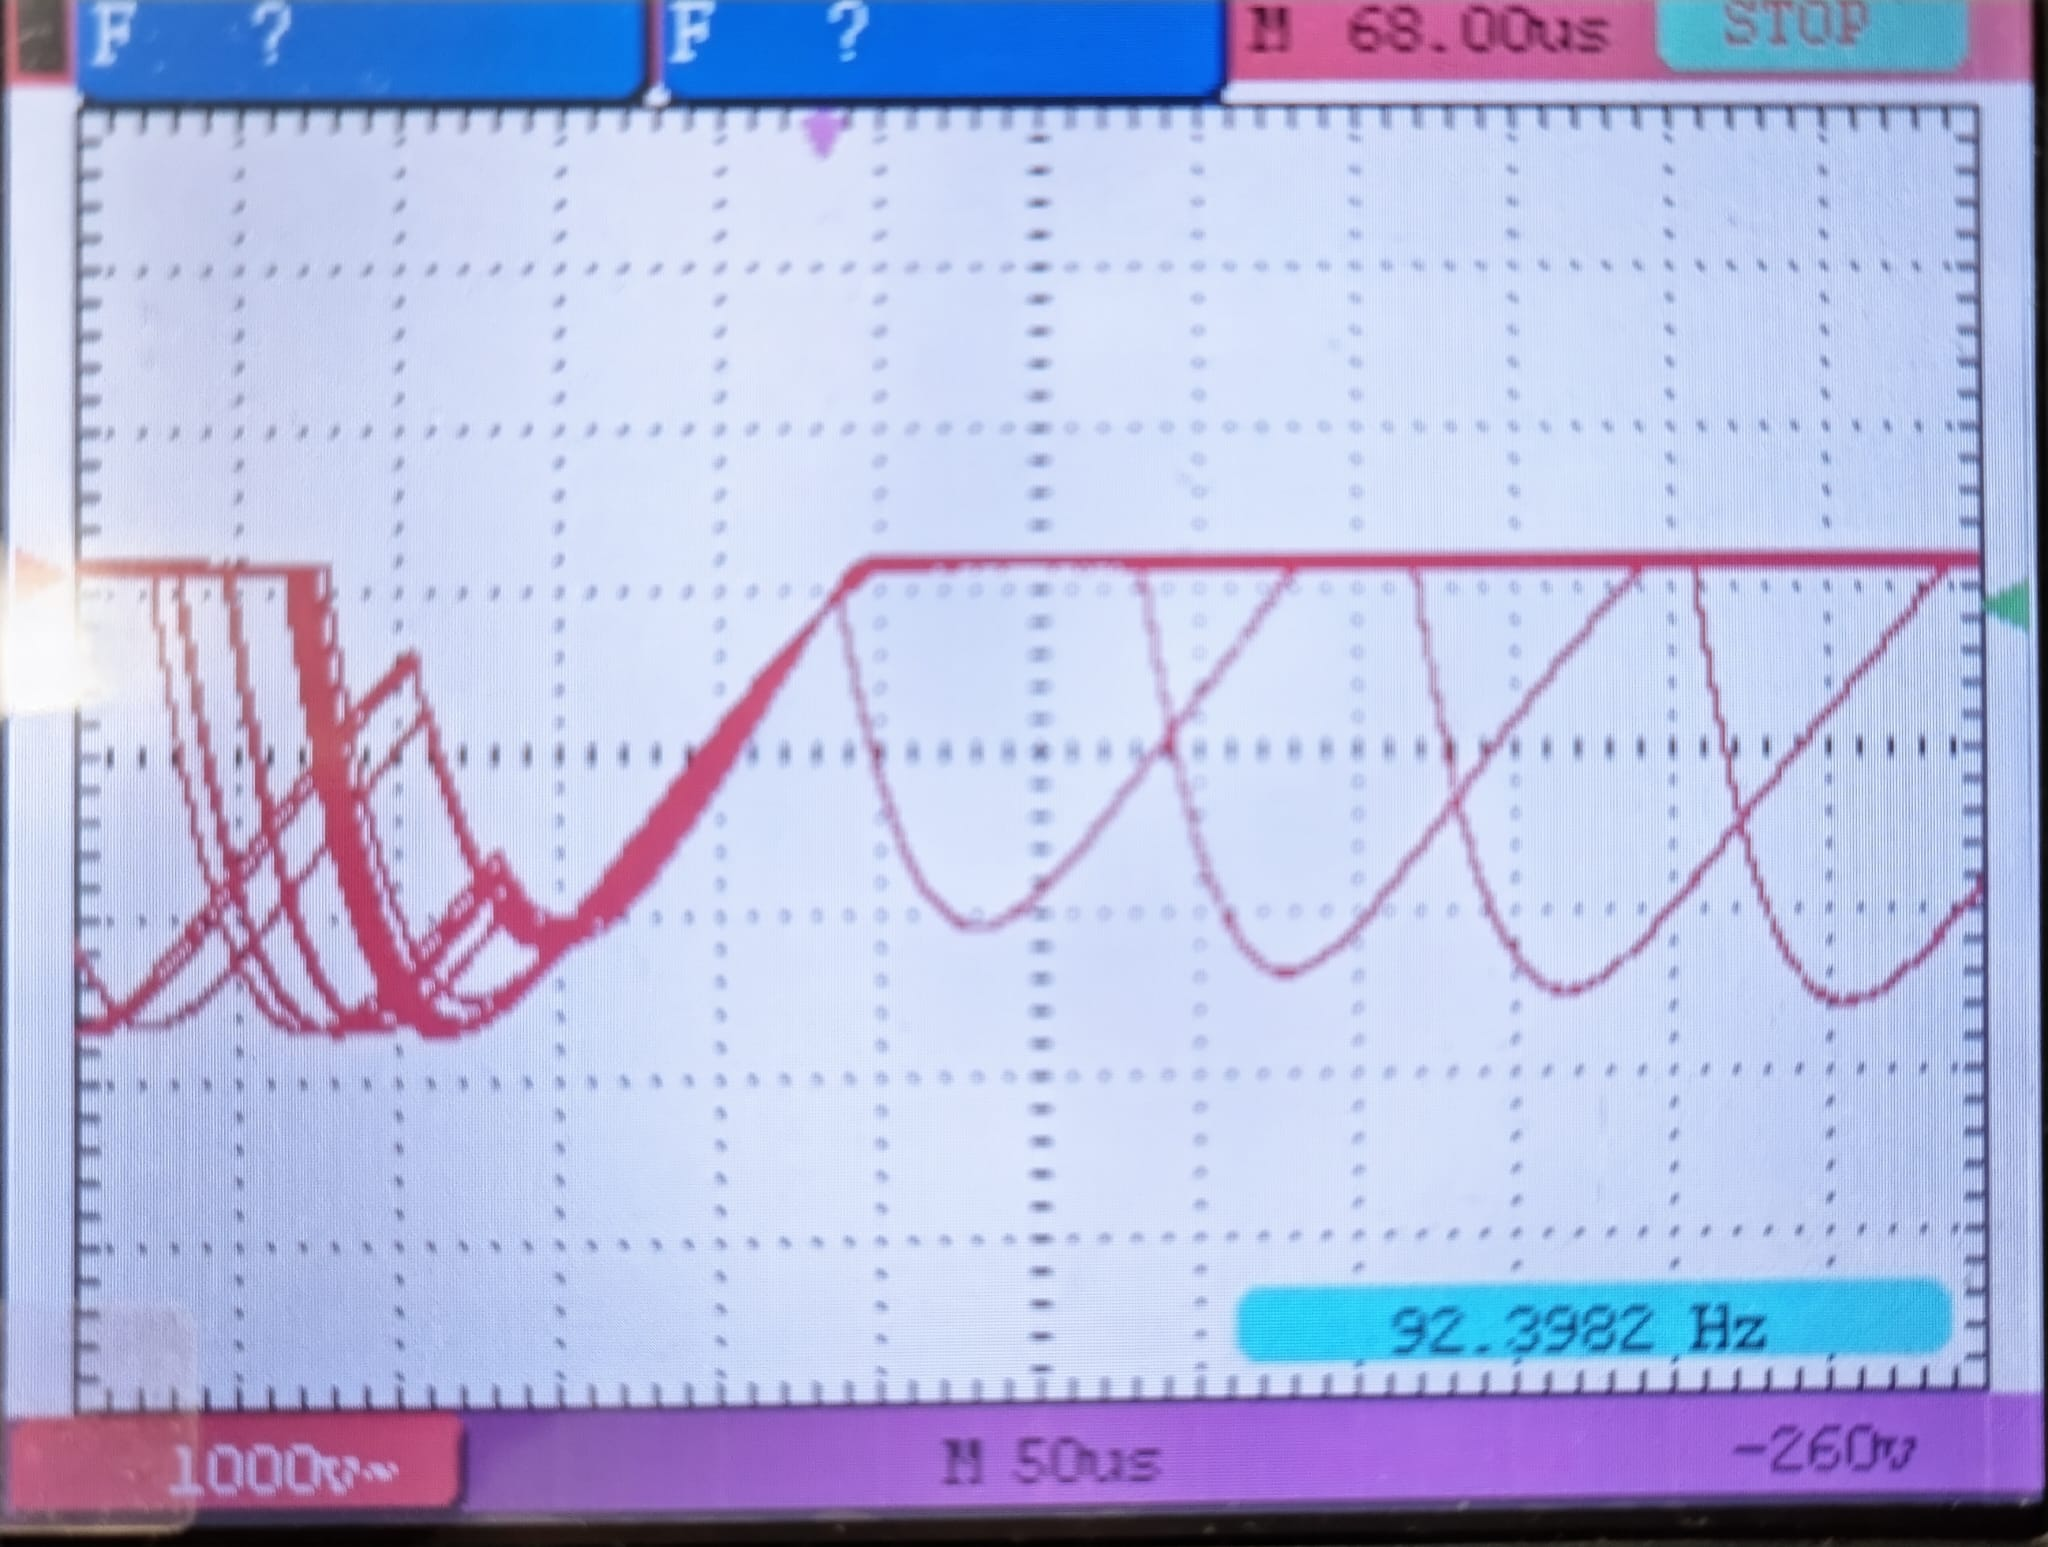
\includegraphics[width = \textwidth]{content/totzeit.jpg}
  \caption{Oszillogramm zur Bestimmung der Totzeit des Geiger-Müller-Zählrohres.}
  \label{fig:totzeit}
\end{figure}

\subsubsection{Zwei-Quellen-Methode}
 Für die Zwei-Quellen-Methode ergeben sich die Messwerte unter Einbezug des 
 Poisson-Fehlers und der Integrationszeit von $120$s zu $N1 = \frac{21844 \pm 148}{120s}$, $N2 = \frac{39105 \pm 198}{120s}$ 
 und $N12 = \frac{17594 \pm 133}{120s}$.\\
 Mit autoref{xxx} berechnet sich die Totzeit zu $T_2 = 253,8 \pm 0,001 \mu$s.




\subsection{Freigesetzte Ladungsmenge}

Die freigesetze Ladungsmenge wird nach autoref{xxx} aus dem mittleren Zählrohrstrom
bestimmt.\\
Sie ist in Abhängigkeit von der Zählrohrspannung in \autoref{fig:lad} graphisch dargestellt.\\
\begin{figure}[H]
  \centering
  \includegraphics{content/figure_2.png}
  \caption{Die freigesetze Ladungsmenge je einfallendem Teilchen in Abhängigkeit von der Zählrohrspannung.}
  \label{fig:lad}
\end{figure}


